% Rapport de stage / Internship report %
%2024-2025 S2 - NORCE %


\documentclass[a4paper, 10pt]{article}

\usepackage[utf8]{inputenc}
\usepackage[french,english]{babel}
\usepackage[T1]{fontenc}
\usepackage{fouriernc}
\usepackage[scaled=0.875]{helvet}
\usepackage{courier}


\usepackage[hidelinks]{hyperref}
\usepackage{fancyhdr}

\pagestyle{fancy}
\setlength{\headheight}{13.59999pt}
\fancyhead[LE]{\thepage}
\fancyhead[RE]{\small \leftmark}
\fancyhead[LO]{\small \rightmark}
\fancyhead[RO]{\thepage}
\fancyfoot[C]{}


\usepackage{graphicx}
\usepackage{tikz}
\usepackage{booktabs}
\usepackage{svg}
\usepackage{picture}
\usepackage{eso-pic}


\usepackage{amsfonts}
\usepackage{amsmath}
\usepackage{amsthm}
\usepackage{multicol}
\usepackage{amssymb}




\begin{document}

    %%% Cover Page %%%


    \AddToShipoutPicture*{%
    \unitlength=1cm
    \put(3.5,19){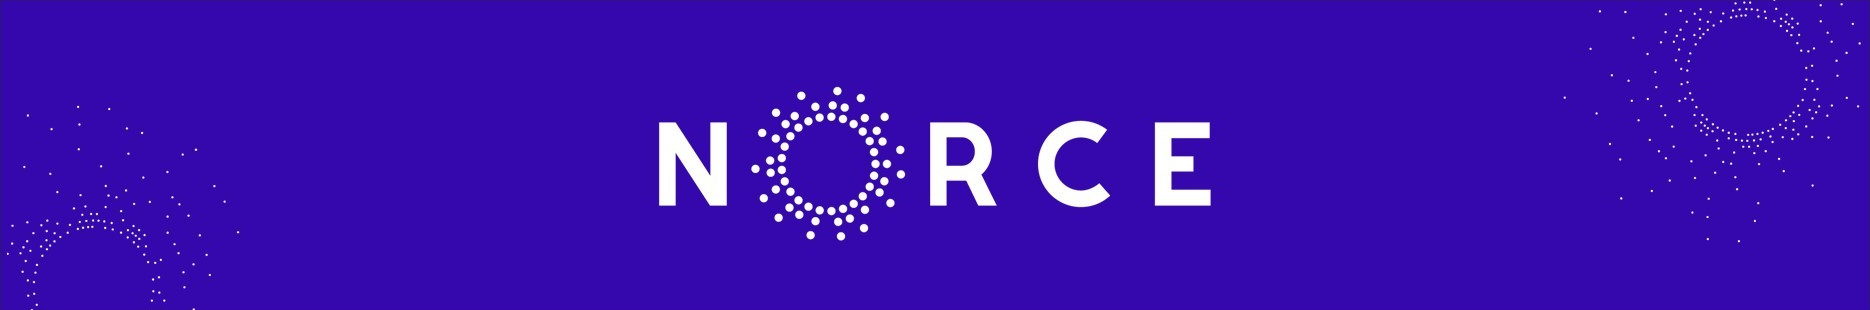
\includegraphics[width=14cm]{img/norce_logo.jpeg}}}


    \thispagestyle{empty}


    \begin{minipage}{0.9\textwidth}
        \centering
        \textbf{\huge Détermination statistique de la fréquence des tempêtes majeures en Norvège par la méthode UNSEEN}
        \vspace{4cm}
    \end{minipage}
    
    \vspace{0.5cm}
    
    \begin{center}
        {\large Émile Sauvat \vspace{10pt} \\ 
        \begin{table}[htbp]
            \centering
            \begin{tabular}{ll}
                \textit{Encadrement :} & \textit{Sigrid Passano Hellan} \\
                & \textit{Étienne Dunn-Sigouin} \\
                & \textit{Erik Kolstad} \\
                \textit{Contact :} & \href{mailto:sipa@norceresearch.no}{\texttt{sipa@norceresearch.no}}
            \end{tabular}
        \end{table}
        }
    \end{center}
    
    \newpage
        
        \setcounter{tocdepth}{3}
    \tableofcontents   
        
    \listoffigures 
    
    \section*{Introduction}


    
\end{document}